\section{Introduction}
\label{sec:intro}
%
Physically accurate simulation of material appearance is an important yet challenging problem, with applications in many areas from entertainment to product design and architecture visualization.
A key ingredient to photorealistic rendering is high-quality material models.
Acquiring the parameters of these models from physical measurements (for example, photographs) has been an active research topic in computer vision and graphics.

Recently, \emph{procedural} material models have been gaining significant traction in the industry (e.g., \cite{Substance}).
In contrast to traditional material reflectance models that represent spatially varying surface albedo, roughness, and normal vectors as 2D images, the procedural models generate such information using a smaller number of user-facing parameters, providing high compactness and easy editability.

In this paper, we introduce a new differentiable computational framework to estimate the parameters of procedural material models.
Our technique enjoys generality by covering a range of materials from standard opaque dielectrics (e.g. plastics, leather, wall paint, wood) to anisotropic brushed metals and metallic paints (Figure~\ref{fig:teaser}). %to scattering media (e.g. milk).
Further, we introduce a novel view of the procedural parameter estimation problem in a \emph{Bayesian framework}, precisely defining prior and posterior distributions of the parameters, allowing for both maximization and sampling of the posterior.

%Our focus on procedural materials is in contrast to several recent methods that estimate parameters separately per pixel. These methods make the assumption of a simple BRDF model (a microfacet specular term, a diffuse term, and a varying normal vector); and their result is in the form of several textures (commonly including diffuse albedo, normal, roughness, and specular coefficient). While the results of the recent methods are impressive, the reality is that procedural materials are gaining significant traction in the industry \cite{Substance}, due to their ability to cover large areas without repetition, easy editability, and small storage requirement.

 \begin{figure*}[t]
 	\centering
 	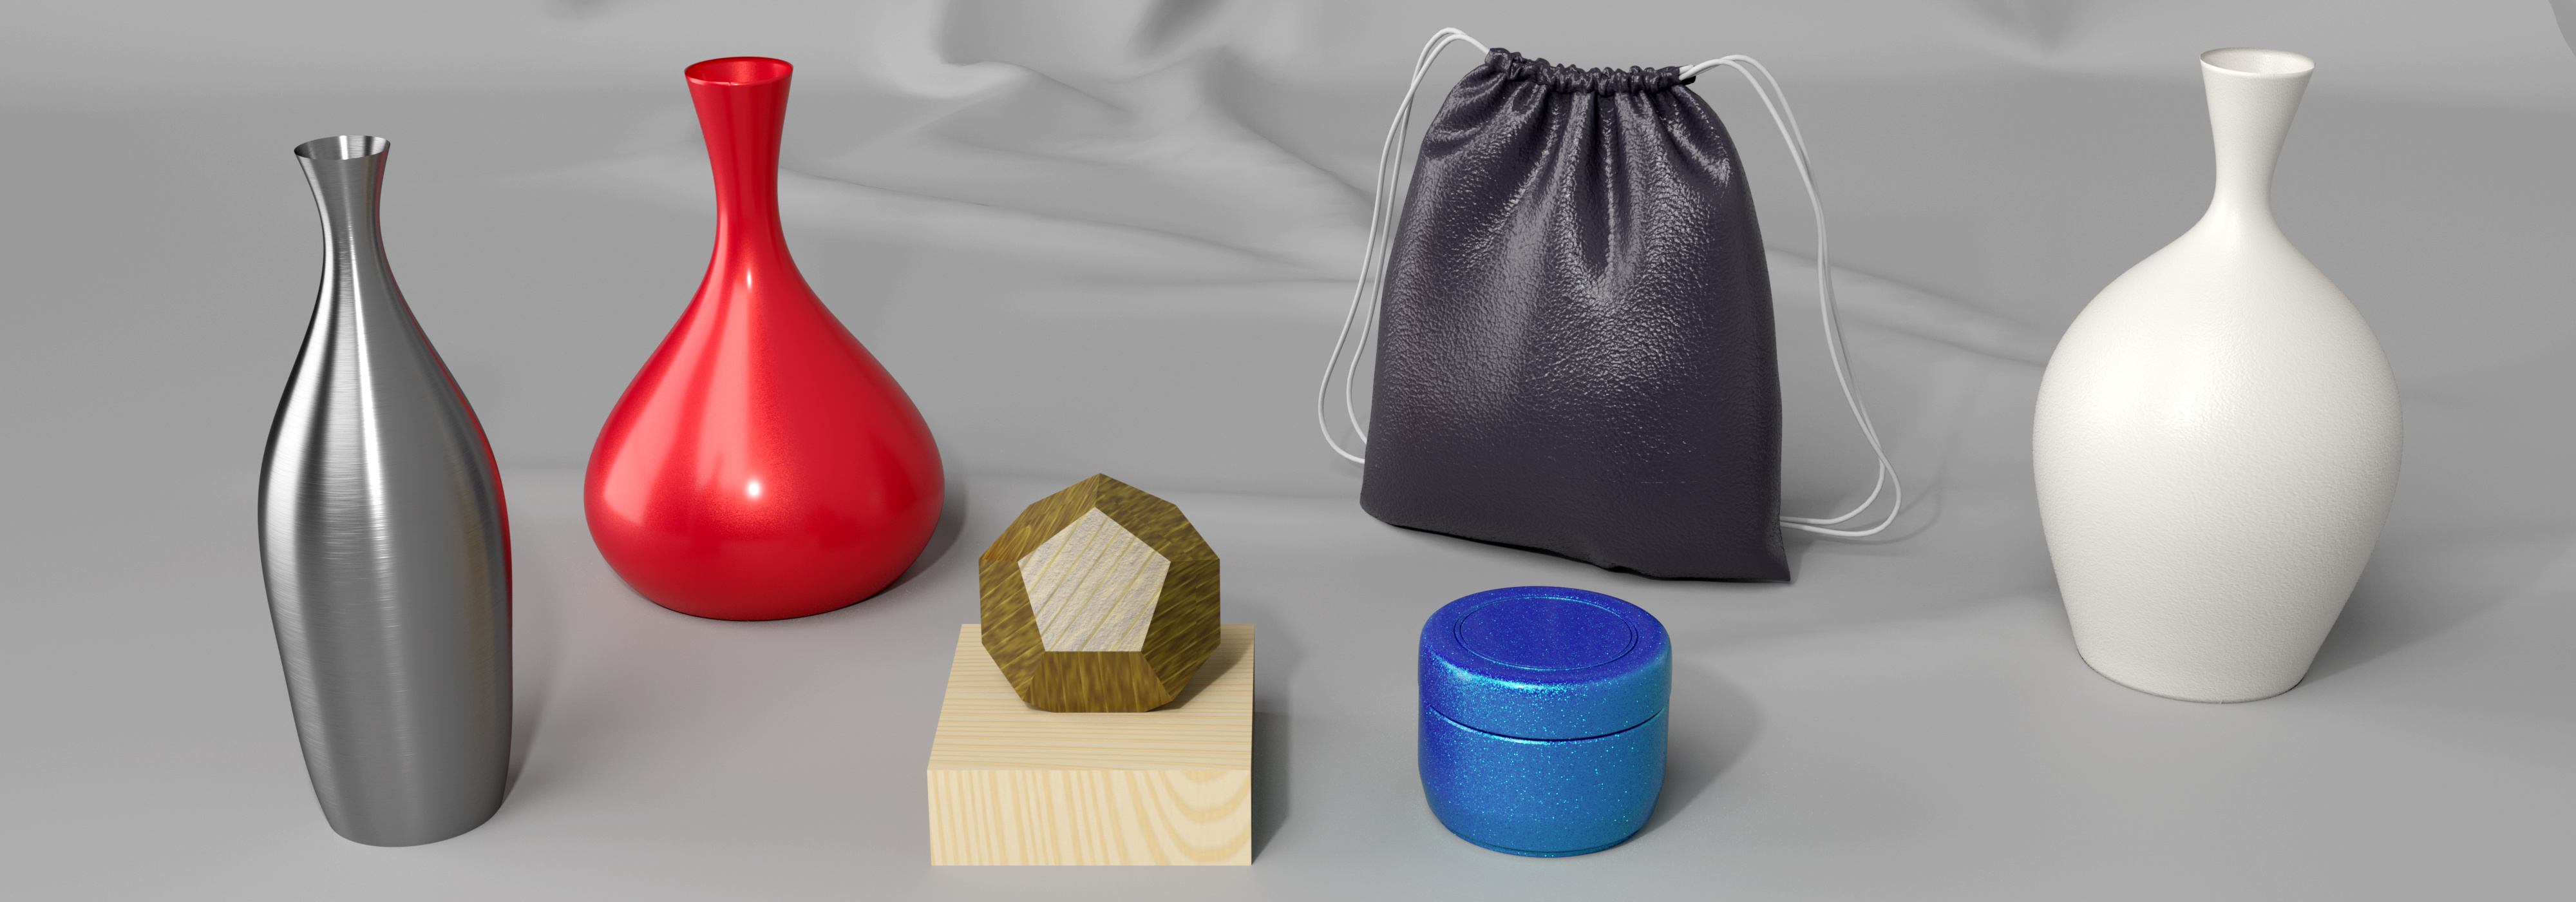
\includegraphics[width=\textwidth]{images/img/teaser.png}
 	\caption{\label{fig:teaser}
 		A scene rendered with material parameters estimated using our method: bumpy dielectrics, leather, plaster, wood, brushed metal, and metallic paint. The insets show a few examples of the initial flash photograph, and our procedural material with parameters found by posterior maximization.
 	}
 \end{figure*}

The estimation of procedural model parameters faces several challenges. First, the procedural generation (and physics-based rendering) of materials is a complex process with a diverse set of operations, making the relationship between procedural model parameters and properties of the final renderings nonlinear and complicated.
Additionally, designing a suitable \emph{loss function} (metric) to compare a synthesized image to a target image is not obvious.
This is because the procedurally generated images do not offer pixel-wise alignments to target images, making simple image difference metrics (e.g., L2 or SSIM) unsuitable.

Our contributions lie in the following two main areas. First, we present a general framework to %address the loss function design problem
compare simulated and target images in a robust fashion without requiring pixel-wise alignments~(\S\ref{sec:summary_func}). To this end, we leverage \emph{summary functions} that map images to latent vectors which can then be compared using L2 or other simple metrics to judge how different two images are.
%A well-designed summary function can be applied to both the simulated and the target image, after which the L2-norm or similar simple metrics can be used to judge the error of a fit.
We consider a number of summary functions, from very simple ones (means of fixed image regions), through higher order statistics and Fourier transforms, to neural summary functions (embeddings) based on Gram matrices of VGG feature maps \cite{Gatys2015,Gatys2016}. The neural embedding approach was first introduced to material capture by Aittala et al. \cite{Aittala2016}; we extend their approach to the case of procedural materials, were it turns out to perform well.

Second, we introduce a \emph{Bayesian inference} approach using Hamiltonian Monte Carlo (HMC) sampling of the space of plausible material parameters~(\S\ref{sec:bayesian}). This provides additional information beyond single point estimates of material parameters (for example, though not limited to, discovering similarity structures in the parameter space). Posterior sampling is a well-studied area within statistics but, to our knowledge, has not yet been applied to material appearance acquisition (or inverse rendering in general).

We implement the procedural generation and rendering processes as (differentiable) PyTorch procedures with the priors and summary functions (classical or neural) expressed in the same framework. These four components (priors, procedural material model, rendering, summary function) together define our posterior distribution (outlined in Figure~\ref{fig:posterior}), a rather complex (but fully differentiable) function.

To demonstrate the efficacy of our techniques, we fit procedural models of a few materials to both synthetic and real target images (\S\ref{sec:results}).

\begin{figure*}[t]
	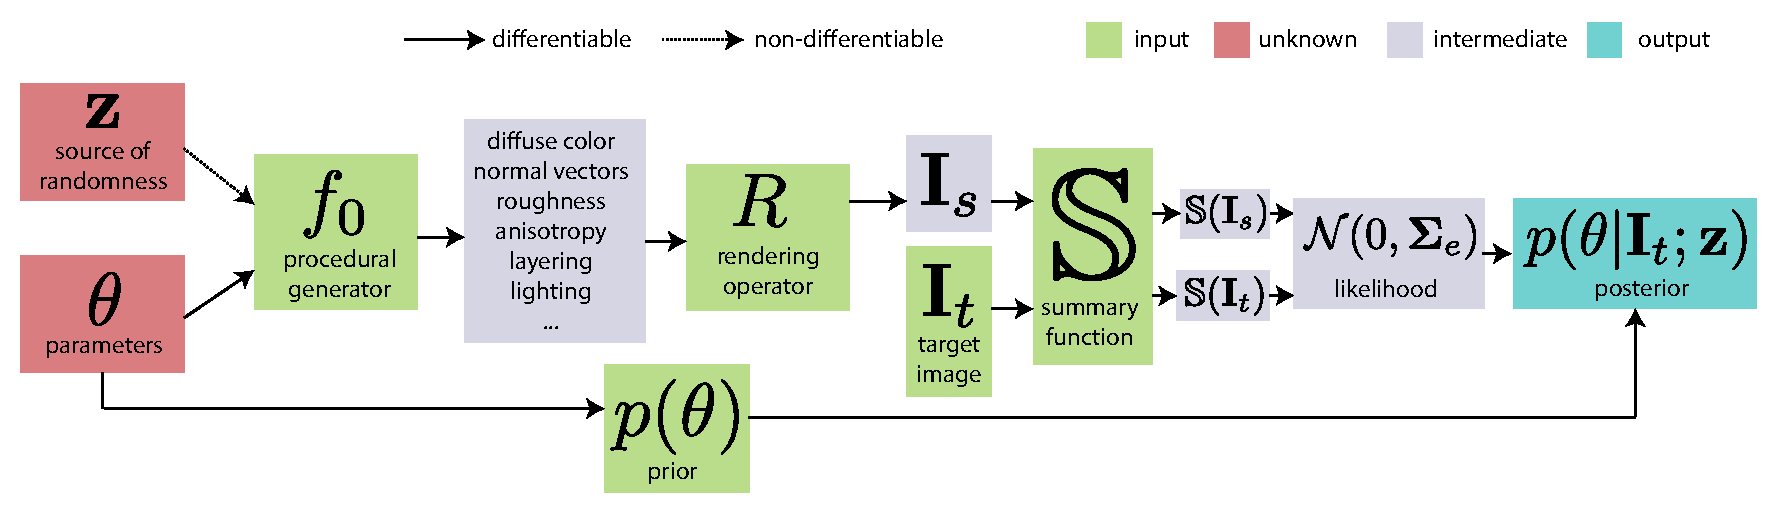
\includegraphics[width=\textwidth]{images/img/posterior.pdf}
	\caption{Our differentiable posterior computation combines priors, a procedural material model, a rendering operator, a summary function, and a target image.}
	\label{fig:posterior}
\end{figure*}
